\subsection{反圆函数}

函数 \(\sin x\) 在区间 \([- \pi/2, +\pi/2]\) 上的限制是严格递增的；其反函数记作 \(\operatorname{Arc}\sin x\) ，它是区间 \([-1, +1]\) 到 \([- \pi/2, +\pi/2]\) 上的严格递增连续映射（图~6）。反函数求导公式（I, p.~9, prop. 6）给出这个函数的导数

\[
\mathrm{D} (\operatorname{Arc} \sin x) = \frac {1}{\cos (\operatorname{Arc} \sin x)}.
\]

由于 \(-\pi/2 \leqslant \operatorname{Arc} \sin x \leqslant \pi/2\) ，有 \(\cos(\operatorname{Arc} \sin x) \geqslant 0\) ；又由于

\[
\sin (\operatorname{Arc} \sin x) = x,
\]

我们有 \(\cos(\operatorname{Arc}\sin x)=\sqrt{1-x^{2}}\) ，由此得

\[
\mathrm{D} (\operatorname{Arc} \sin x) = \frac {1}{\sqrt {1 - x ^ {2}}}.\tag{16}
\]

同样，\(\cos x\) 在区间 \([0, \pi]\) 上的限制是严格递减的；其反函数记作 \(\operatorname{Arc}\cos x\) ，它是 \([-1, +1]\) 到 \([0, \pi]\) 上的严格递减映射（图~6）。此外

\pandocbounded{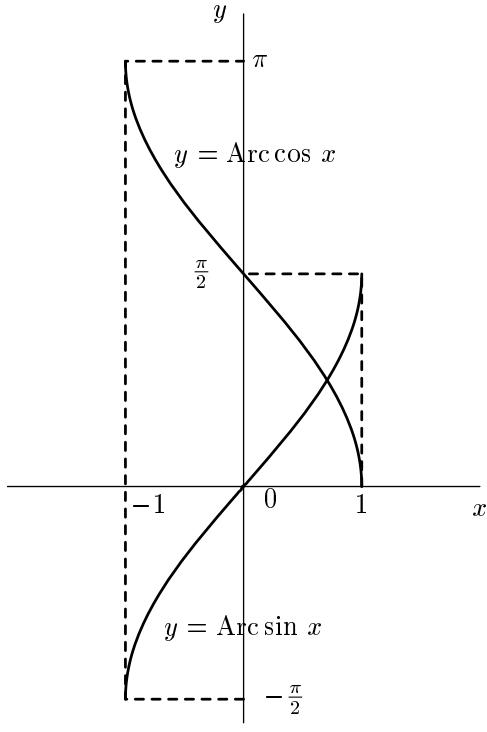
\includegraphics[keepaspectratio]{images/part001_f987f09f.jpg}}\\
图 6

\[
\sin \left(\frac {\pi}{2} - \operatorname{Arc} \cos x\right) = \cos (\operatorname{Arc} \cos x) = x
\]

并且由于 \(-\pi / 2 \leqslant \pi / 2 - \operatorname{Arc} \cos x \leqslant \pi / 2\) ，有

\[
\operatorname{Arc} \cos x = \frac {\pi}{2} - \operatorname{Arc} \sin x\tag{17}
\]

特别由此得出

\[
\mathrm{D} \big (\operatorname{Arc} \cos x \big) = - \frac {1}{\sqrt {1 - x ^ {2}}}.\tag{18}
\]

最后，\(\tan x\) 在区间 \(]-\pi/2, +\pi/2[\) 上的限制是严格递增的；其反函数记作 Arc \(\tan x\) ，它是 R 到 \(]-\pi/2, +\pi/2[\) 上的严格递增映射（图~7）；我们有

\[
\lim _ {x \rightarrow - \infty} \operatorname{Arc} \tan x = - \frac {\pi}{2}, \quad \lim _ {x \rightarrow + \infty} \operatorname{Arc} \tan x = \frac {\pi}{2},
\]

并且，应用反函数求导公式以及 III, p.~95 的公式 (15)，有

\[
\mathrm{D} \big (\operatorname{Arc} \tan x \big) = \frac {1}{1 + x ^ {2}}.\tag{19}
\]

\pandocbounded{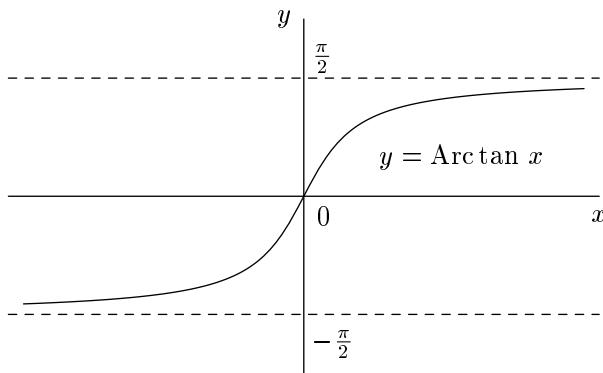
\includegraphics[keepaspectratio]{images/part001_f81b3ea6.jpg}}\\
图 7

